\section{Laboratory work implementation}

\subsection{Tasks and Points}
\begin{itemize}
\item \textbf{Basic Level (grade 5 - 6) you should be able to:}
	\begin{enumerate}
	\item Created a Window's application
      \item Presented in the middle of the window the text "Done with Pride and Prejudice by student name". Replaced student name with my name.
      \item On windows resize, text reflow and be in window's middle (vertically and horizontally)
      \end{enumerate}
\item \textbf{Normal Level (grade 7 - 8) you should be able to:}
      \begin{enumerate}
    \item Realized the tasks from \textit{Basic Level}.
    \item Added a button on the window with default styles.
    \item Added a button on the window with custom size.
    \item Added 2 text elements to window: one with default styles, one with custom styles (size, background, text color, font family/size)
          \end{enumerate}
\item \textbf{Advanced Level (grade 9 - 10) you should be able to:}
      \begin{enumerate}
    \item Realized the tasks from \textit{Normal Level}.
    \item I got the text from one text element on button click  and placed into another 
    \item Made 2 buttons disappeared on a button click
    
    \item The window took different colors on re-size
    \item	  The window took the blue color on moving it over desktop
    \item    The window didn't close on pressing the close button , it threw a info alert where it's described how to close it.
          \end{enumerate}
  \end{itemize}  


\subsection{Laboratory work analysis}

Add link to your repository.
Create a README.md file for each laboratory work you submit. It should include the tasks that you had been implemented.
Explain the features that you had been added to your window.

\subsection{Prove your work with screens}

\begin{figure}[h!]
  \centering
    {%
      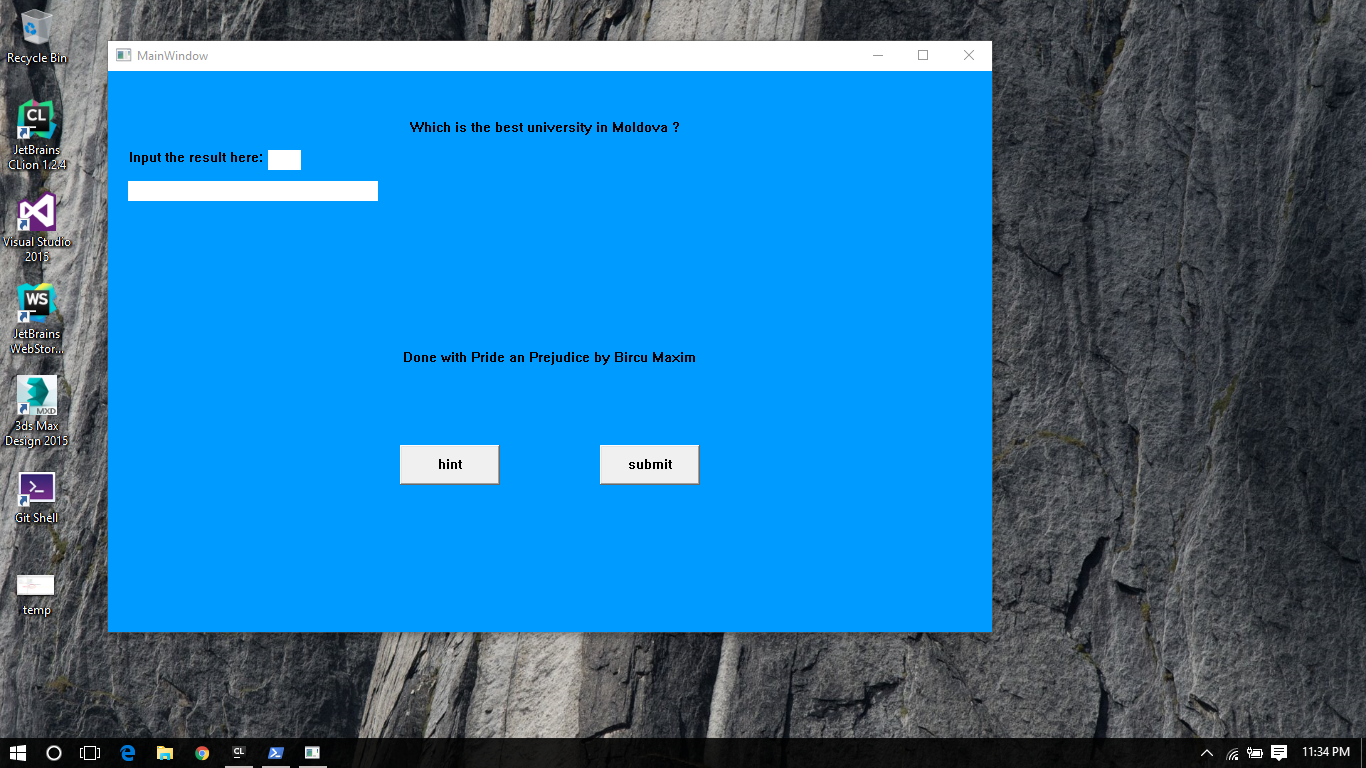
\includegraphics[width=0.5\textwidth]{screen1}}
  \caption{Window is open}
\end{figure}

\begin{figure}[h!]
  \centering
    {%
      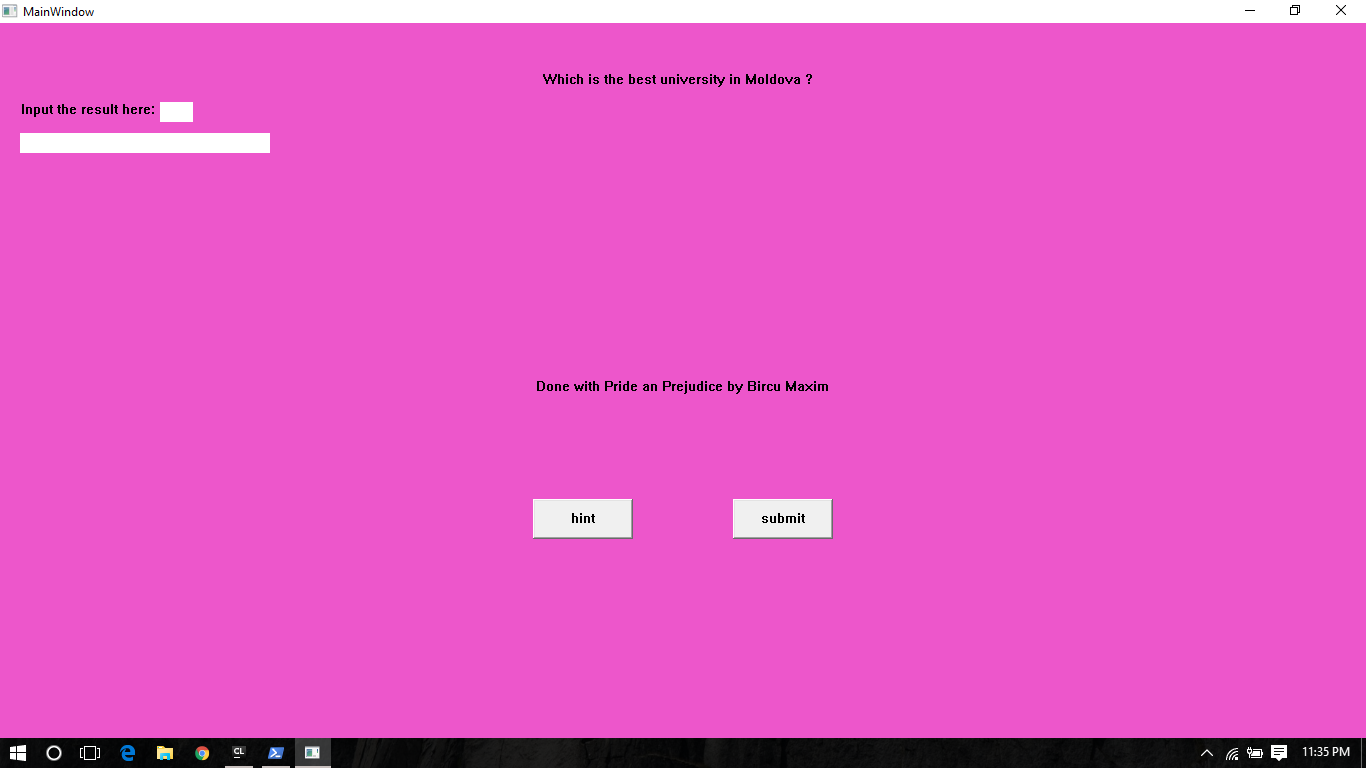
\includegraphics[width=0.5\textwidth]{screen2}}
  \caption{Full screen window}
\end{figure}

\begin{figure}[h!]
  \centering
    {%
      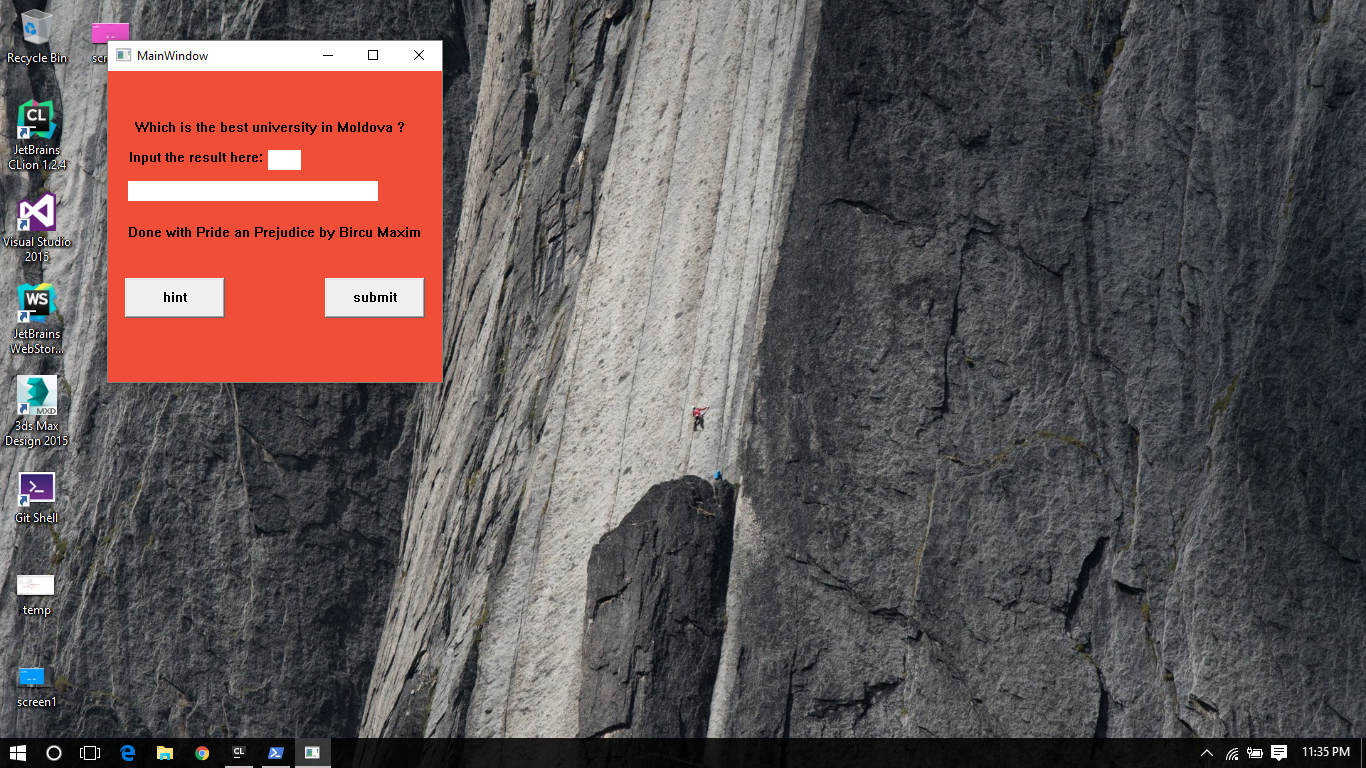
\includegraphics[width=0.5\textwidth]{screen3}}
  \caption{Min size window}
\end{figure}

\begin{figure}[h!]
  \centering
    {%
      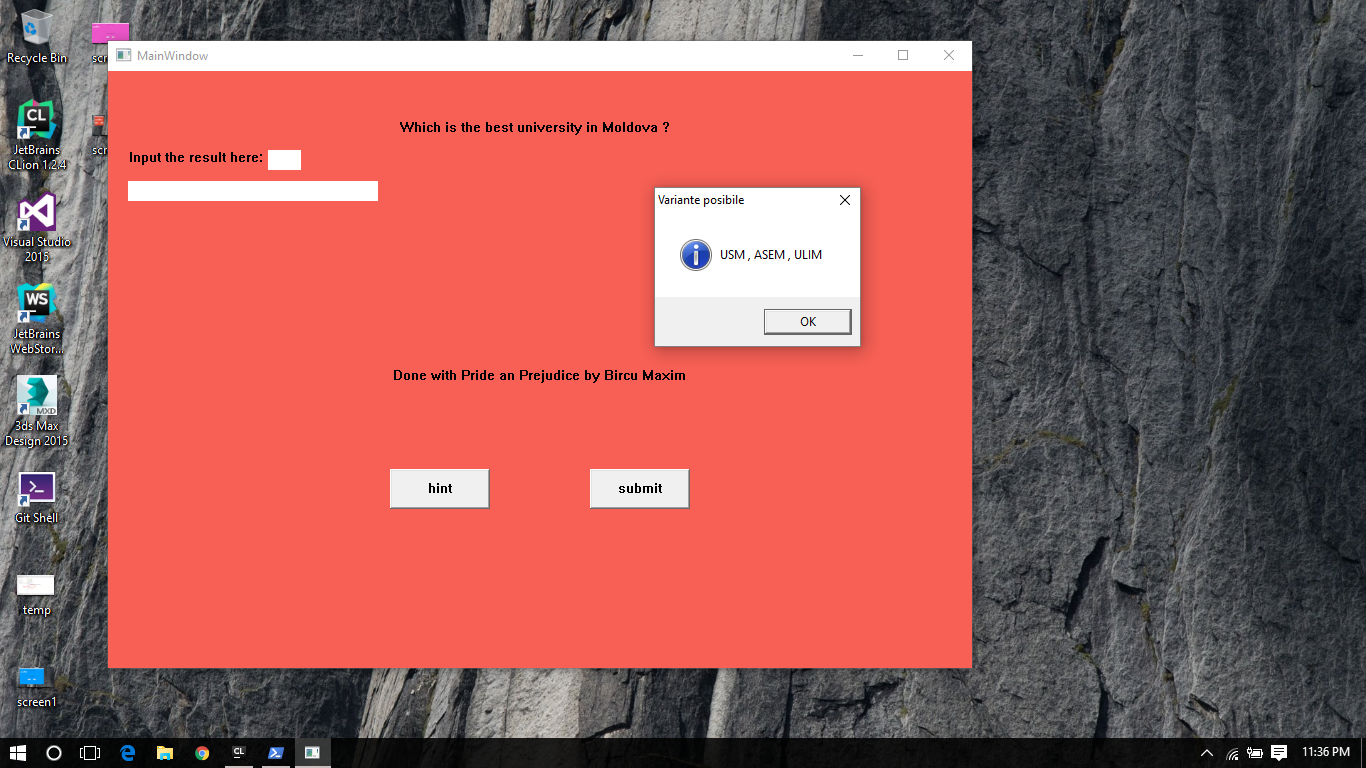
\includegraphics[width=0.5\textwidth]{screen4}}
  \caption{Message with hints}
\end{figure}

\begin{figure}[h!]
  \centering
    {%
      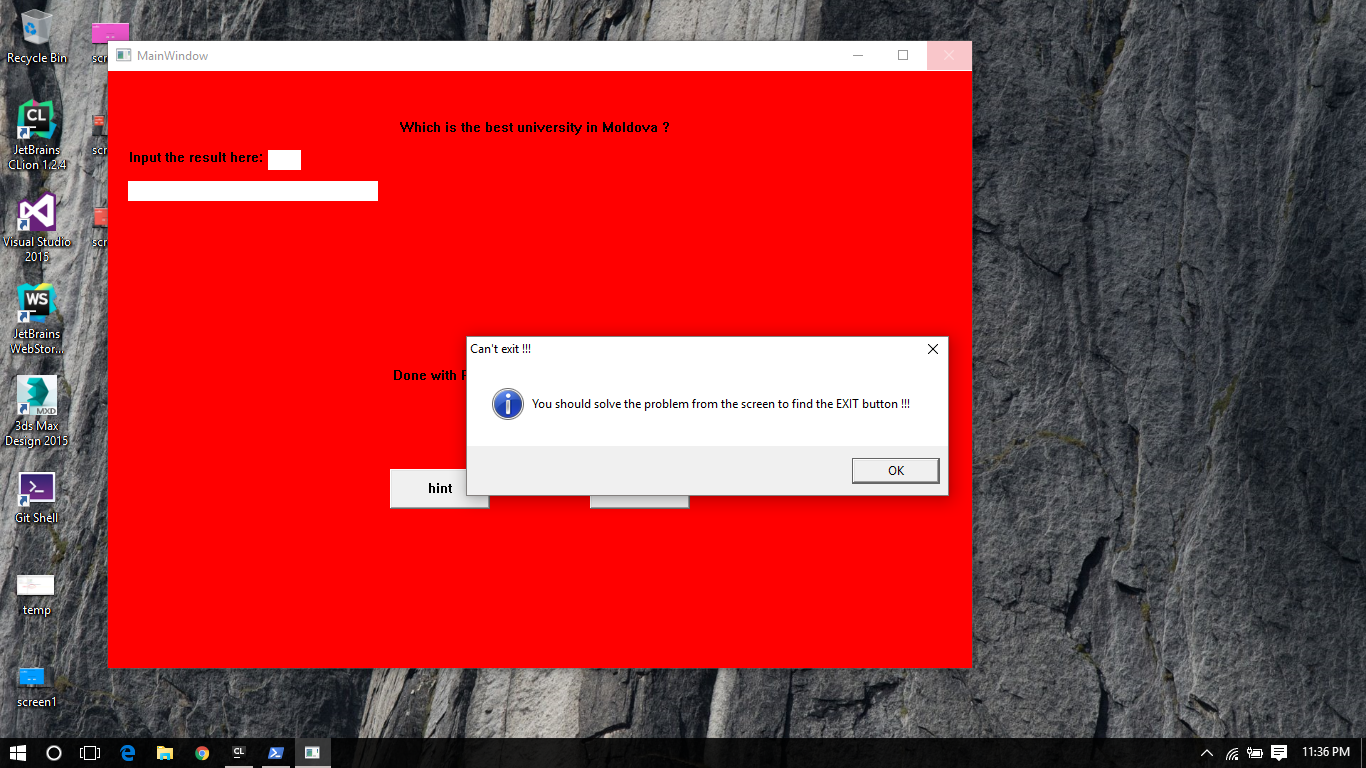
\includegraphics[width=0.5\textwidth]{screen5}}
  \caption{Message can't close window}
\end{figure}

\begin{figure}[h!]
  \centering
    {%
      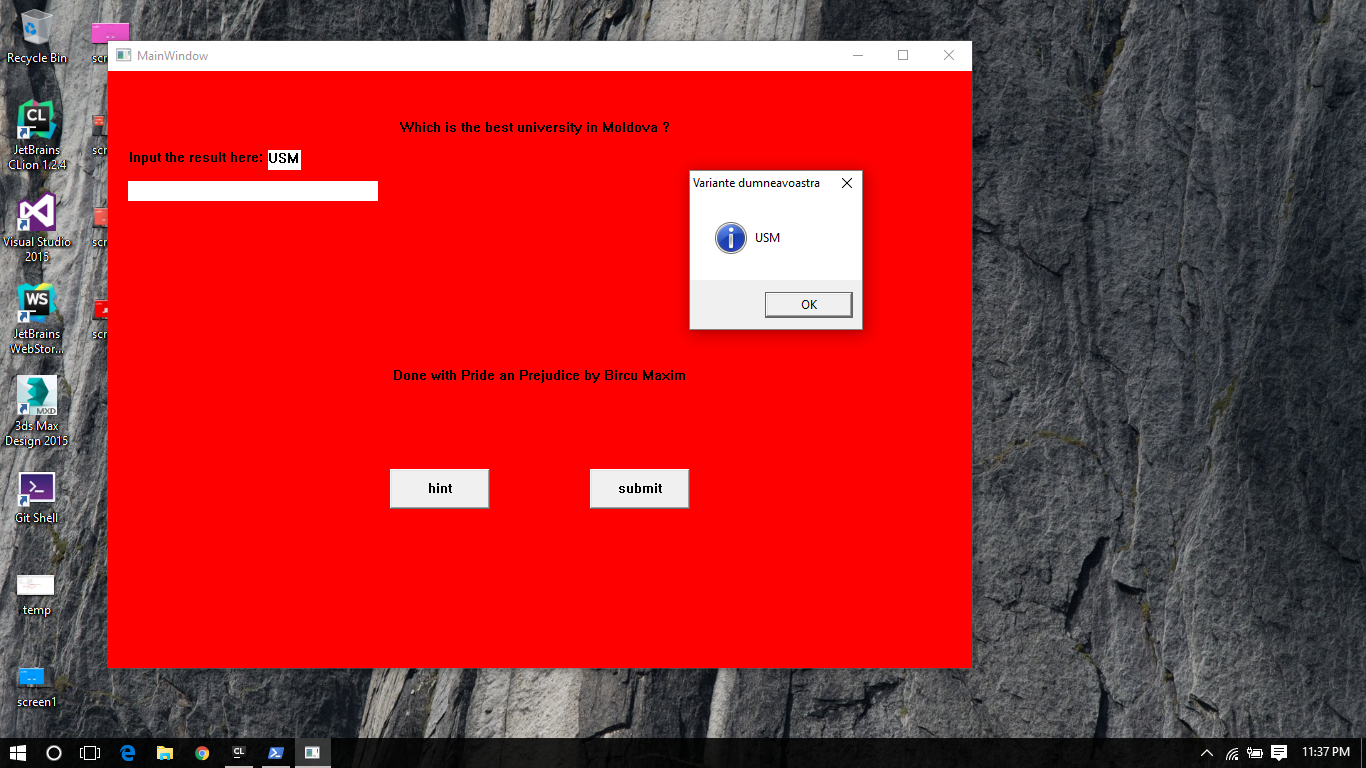
\includegraphics[width=0.5\textwidth]{screen6}}
  \caption{Trying to chose a solution}
\end{figure}

\begin{figure}[h!]
  \centering
    {%
      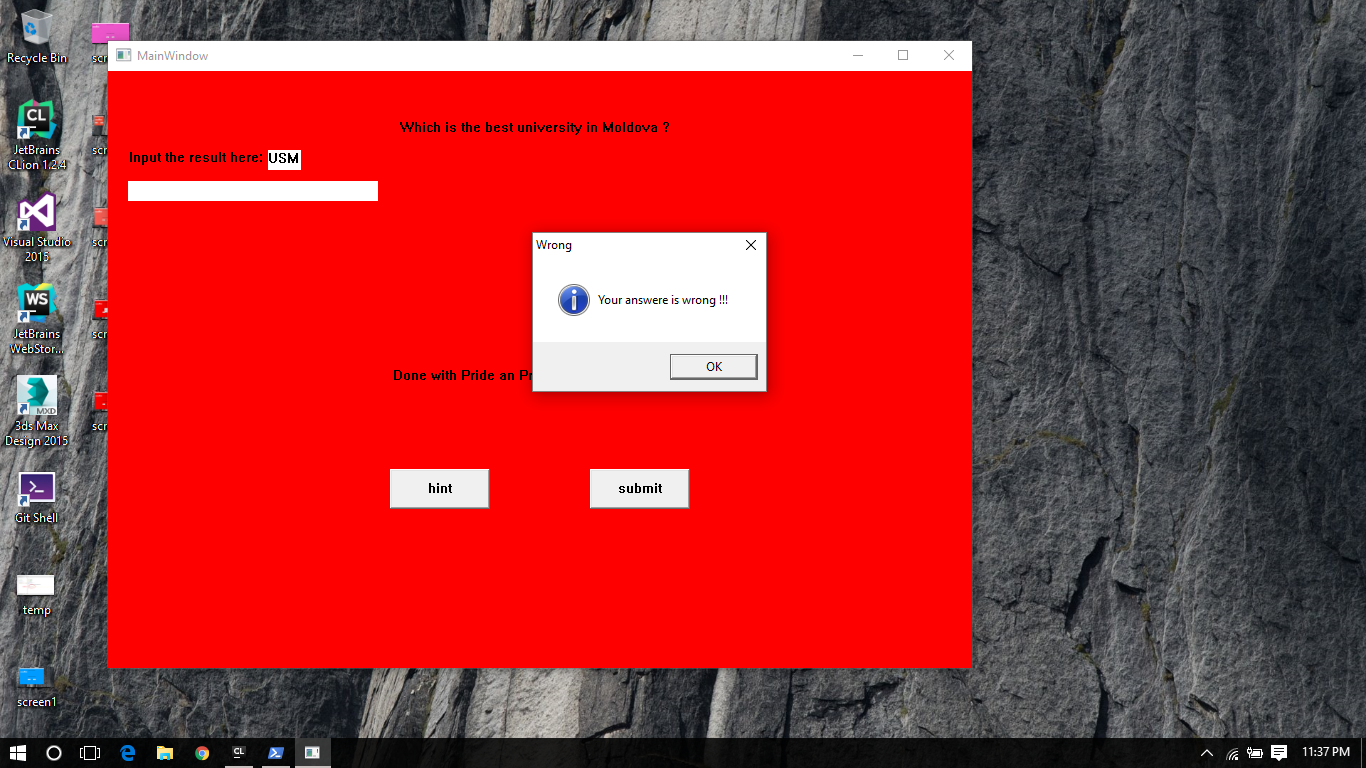
\includegraphics[width=0.5\textwidth]{screen7}}
  \caption{The solution is not correct}
\end{figure}

\begin{figure}[h!]
  \centering
    {%
      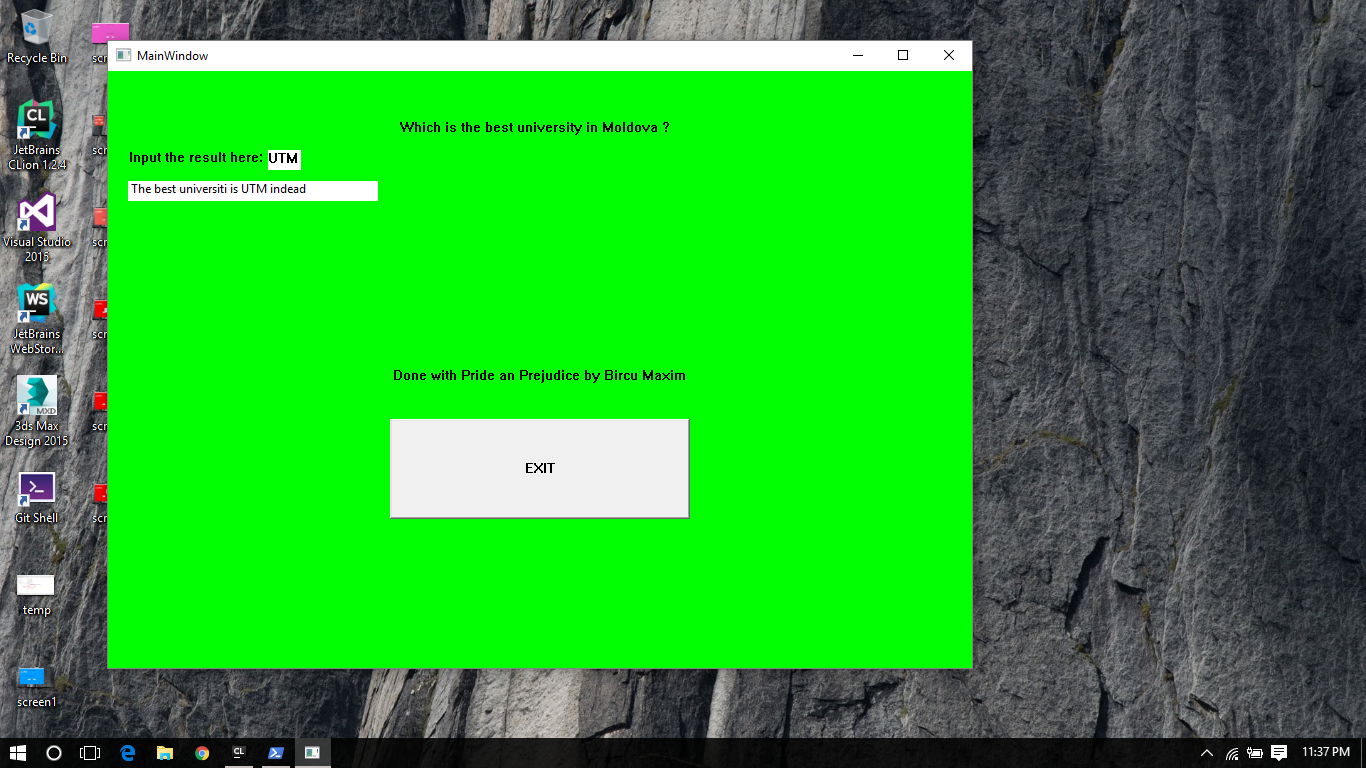
\includegraphics[width=0.5\textwidth]{screen8}}
  \caption{The solution is correct and window can be close}
\end{figure}
\clearpage